\documentclass[11pt]{exam}

\usepackage{listings}
\usepackage{graphicx}


\lstdefinestyle{latexsty}{
	language={[LaTeX]TeX},
    basicstyle=\small\ttfamily,
    breaklines=true,
    breakindent=0pt, 
    numbers=left, stepnumber=1, numbersep=5pt,
    commentstyle=\color{red},
    showstringspaces=false,
    %keywordstyle=\color{blue}\bfseries,
    morekeywords={align,begin},
    tabsize=2,
    frame=single,
}

\pagestyle{headandfoot}
\runningheader{\LaTeX: An Introduction (Part 1)}{Exercise 1}{10th February 2014}
\runningheadrule
\runningfooter{}{\thepage}{}
\runningfootrule

\title{Exercise 1 - Running \LaTeX, Editing \& Compiling \LaTeX\ Documents}
\author{UGC `\LaTeX: An Introduction (Part 1)' Training Course}
\date{February 10th 2014}

\begin{document}
\maketitle

\fbox{\parbox{0.9\textwidth}{The USB drive you have been given contains a portable distribution of MiKTeX for Windows, which can be run directly from the USB drive with no installation required. \emph{Please return the drive at the end of the day, it is needed for another course!}}}

\vspace{0.2in}

In order to run MiKTeX, open the folder on the USB drive entitled \texttt{Miktex} and run (double click) on the file named \texttt{miktex-portable.cmd}. This will place a MiKTeX icon in the system notification tray, as in Figure~\ref{fig:trayicon}. From this icon you can set MiKTeX options, open a command prompt to compile \LaTeX\ files from the command line, or start TeXworks -- the text editor provided with MiKTeX for editing \LaTeX.

\begin{figure}[htbp]
	\centering
	\fbox{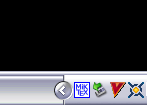
\includegraphics{img/desktop.PNG}}
	\caption{MiKTeX icon in System Tray}
	\label{fig:trayicon}
\end{figure}


\begin{questions}

\question
Right-click on the MiKTeX tray icon and select `\texttt{TeXworks}'. After a short time, the \texttt{TeXworks} editor should open as in Figure~\ref{fig:texworks}.

\begin{figure}[htbp]
	\centering
	\fbox{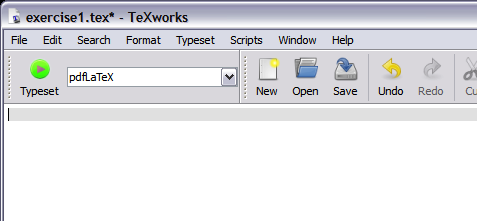
\includegraphics[width=0.5\textwidth]{img/texworks.PNG}}
	\caption{TeXworks window}
	\label{fig:texworks}
\end{figure}



\uplevel{The green icon in the top-left corner of the window will compile and display your \LaTeX\ files. The drop-down box next to it allows you to select the \LaTeX\ compilation method you wish to use. We are creating simple \LaTeX\ documents, so there is no need to run \texttt{makeindex} or \texttt{bibtex} when compiling our documents.}
\question
If it is not already selected, choose `\texttt{pdflatex}' in the drop down box.
\question
Save your file somewhere in your filespace with a suitable name (something like \texttt{exercise1.tex} perhaps?).
\uplevel{We are now ready to start creating our first \LaTeX\ document.}
\question
Enter the \LaTeX\ code below:


\begin{lstlisting}[style=latexsty]
	\documentclass{article}
	\begin{document}
		Hello World!
	\end{document}
\end{lstlisting}

\question
Click the green arrow to compile your document. The console output window will show you the process of \LaTeX\ compilation, then the resulting \texttt{.pdf} file will be displayed. Hopefully, it should look like Figure~\ref{fig:output}

\begin{figure}[htbp]
	\centering
	\fbox{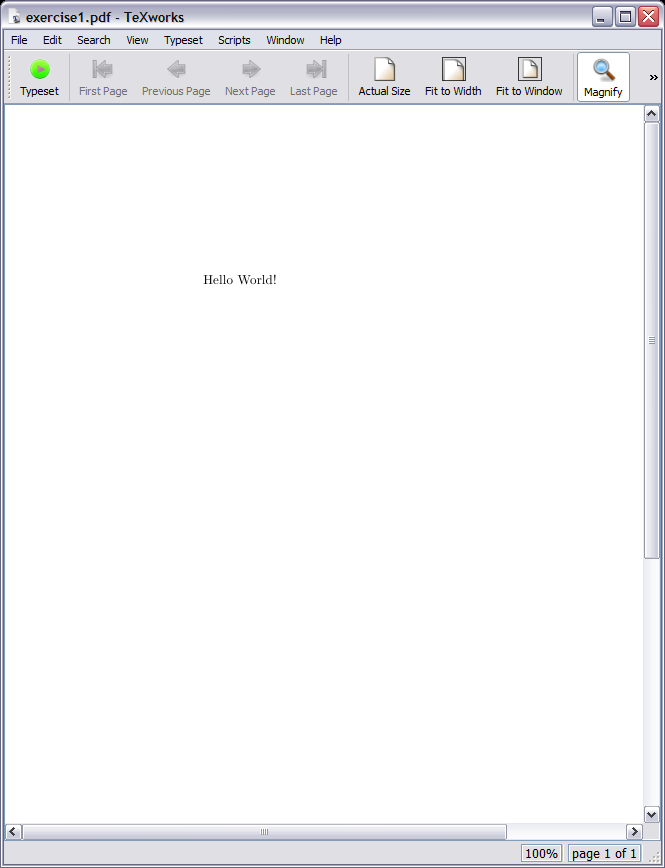
\includegraphics[width=0.5\textwidth]{img/output.PNG}}
	\caption{Completed Output}
	\label{fig:output}
\end{figure}

\uplevel{Congratulations! You just edited and compiled your first \LaTeX\ document!}

\end{questions}

\end{document}